\documentclass[10pt,a4paper,oneside,twocolumn]{article}

    \usepackage{float}	% for floating figures (putting them anywhere we want
    \usepackage{amsmath}	% for maths
    \usepackage{graphicx}	% jpg
    \usepackage{hyperref}
    \usepackage{textcomp}
    \usepackage{verbatim}	% use of \begin{comment}
    \usepackage{pgfplots}	% use of pgf plots
    \usepackage{multicol}
  %  \usepackage[top=2cm, bottom=2cm, left=2cm, right=2cm]{geometry} %margins
    \usepackage{sidecap}	% for side captions
    \restylefloat{table}	% floating figures(Tables)
    \usepackage{caption}
    \captionsetup{justification=justified}
    \usepackage{subcaption}

    \numberwithin{equation}{section} %permits numbering within sections instead of globally
\begin{document}

\title{\huge{\textbf{Report}}\\
	\vspace{0.5cm}
	\Large{\textit{\'Ecole Polytechnique F\'ed\'erale de Lausanne, Switzerland}}}
\author{\large{Florian + Dariush}}

\begin{titlepage}
 \maketitle
\thispagestyle{empty}
\end{titlepage}

\section{Introduction}
    Introduction to the article goes here \\
\section{The Model}

    \begin{figure}[!h]
	\centering
	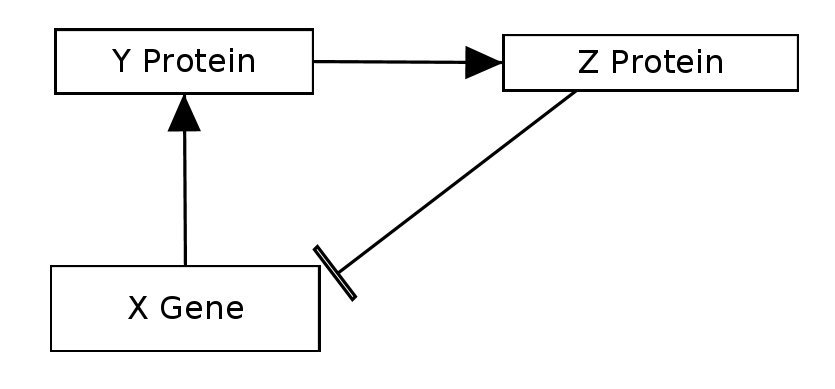
\includegraphics[scale=0.3]{sketch.png}
	\caption{Sketch of that thing blabla}
    \end{figure}
    
    b/ablalaeolauelthaeou

    \begin{figure*}[!h]
	\begin{subfigure}[b]{0.5\textwidth}
	    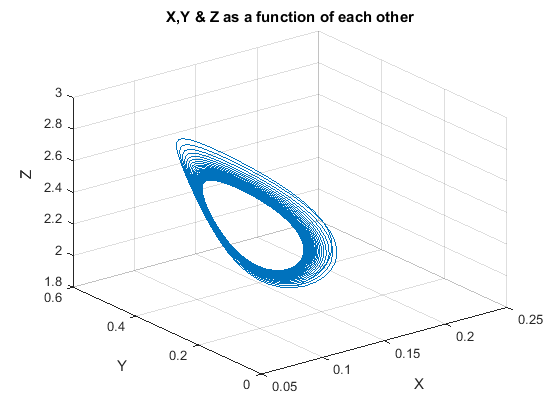
\includegraphics[width=\textwidth]{A11.png}
	    \caption{A gull}
	    \label{fig:gull}
	\end{subfigure}
	~ %add desired spacing between images, e. g. ~, \quad, \qquad, \hfill etc. 
	  %(or a blank line to force the subfigure onto a new line)
	\begin{subfigure}[b]{0.5\textwidth}
	    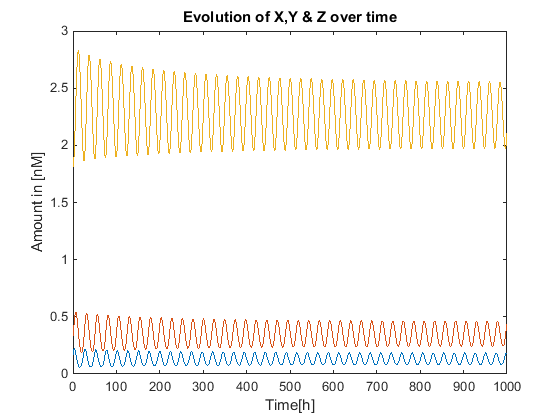
\includegraphics[width=\textwidth]{A12.png}
	    \caption{A tiger}
	    \label{fig:tiger}
	\end{subfigure}
    \end{figure*}

\end{document}
